\documentclass[a4paper]{llncs}
\usepackage{comment}
\usepackage{printlen} % Print lengths using specified units. 
%\usepackage{hyperref}
\usepackage{booktabs}
\usepackage[utf8]{inputenc} % Umlaute üöä auch normal benutzen und nicht maskieren
\usepackage{color}
% http://www.ctan.org/tex-archive/fonts/ps-type1/cm-super/
\usepackage[T1]{fontenc} % use high quality fonts, please install cm-super
\usepackage[pdftex]{graphicx}
\graphicspath{{./Depictions/}}
\DeclareGraphicsExtensions{.pdf,.jpeg,.jpg,.png}
\usepackage[T1]{url}
\usepackage{listings}
\usepackage{subfig}
\usepackage{printlen} % Print lengths using specified units.
\usepackage{booktabs}
%\usepackage[textsize=tiny]{todonotes}
\usepackage{todonotes}

\usepackage[
pdftex,
bookmarks=true,
hidelinks,
unicode=true,
pdfauthor={Sebastian Tramp, Henry Story, Philipp Frischmut, Timofey Ermilov, and S\"oren Auer},
pdftitle={Extending the WebID Protocol with Access Delegation},
pdfkeywords={WebID, Social Semantic Web, Access Delegation}
]{hyperref}

\title{Extending the WebID Protocol with Access Delegation}

\author{Sebastian Tramp\inst{1} \and Henry Story\inst{2} \and Philipp Frischmuth\inst{1} \and Timofey Ermilov\inst{1} \and S\"oren Auer\inst{1}}

\institute{
Universit\"at Leipzig, Institut f\"ur Informatik, AKSW,\\
Postfach 100920, D-04009 Leipzig, Germany,\\
\email{\{lastname\}@informatik.uni-leipzig.de}\\
\url{http://aksw.org/FirstnameLastname} (WebID)
\medskip\and
Apache Foundation\\ 
\email{henry.story@bblfish.net}\\
\url{http://bblfish.net/people/henry/card\#me} (WebID)
}

\authorrunning{Sebastian Tramp et al.}

%%%%% LISTINGS
\usepackage{listings} % Typeset source code listings using LaTeX.
% listing styles
\lstset{%
    numberbychapter=false,
    numberblanklines=true,
    numbers=left,
    numberstyle=\tiny,
    basicstyle=\ttfamily\footnotesize,
    emphstyle=\textit,
    tabsize=2,
    framexleftmargin=2pt,
    captionpos=b,
    frame=single,
    breaklines=true
}
\lstdefinestyle{rdf}{morekeywords={}}
\lstdefinestyle{sparql}{
    morekeywords={SELECT,OPTIONAL,FROM,DISTINCT,a,WHERE,FILTER,GROUP,ORDER,LIMIT,BY,IN,AS},
    emph={s,p,o}
}
\lstdefinestyle{turtle}{
    morekeywords={a, @prefix, cert,xsd,foaf, rdf, rdfs, owl},
    morecomment=[s][\textrm]{<}{>},
    morecomment=[s][\textit]{"}{"},
}

\begin{document}

\maketitle              % typeset the title of the contribution

\begin{abstract}
We propose \ldots
\end{abstract}

\section{Introduction and Terminology}\label{sec:intro}

% this prints the current textwidth, so images can be
% generated perfectly fitting to the page (LNCS textwidth: 121.99854 mm)
%\uselengthunit{mm}\printlength{\textwidth}
%\uselengthunit{mm}\printlength{\columnwidth}

\cite{story-h-2009--a}
\cite{tramp-s-2012--a}

%\begin{figure}[!t]
%\centering
%\includegraphics[width=2.5in]{myfigure}
%\caption{Simulation Results}
%\label{fig_sim}
%\end{figure}



A \textit{WebID} is a URI that refers to an Agent - Person, Robot, Group or other thing that can have Intentions.
The WebID should be a URI which when dereferenced returns a representation whose description uniquely identifies the Agent as the controller of a public key~\cite{sporny-m-2011--a}.
As a non-exclusive alternative, we propose that this description can also refer to a secretary agent WebID for access delegation.
This allows even for WebID descriptions which do not control a public key itself and only delegate access to other WebIDs (refer to \autoref{sec:WorkingGroups}).

In the context of access delegation, we distinguish a WebID which refers to an agent which has direct access to a certain resource from a WebID which refers to an agent which has access to a resource only if he acts in the name of the first agent.
We call the latter agent the \textit{secretary agent} and the first one the \textit{named agent}.
\todo{maybe another name here?}

\textit{Access Delegation} is a relation between two WebID resources.
The relation describes, under which circumstances a secretary agent has access to a certain resource under the same constraints as the named agent.
The secretary agent declares to act in the name of the named agent.

\section{Requirements}

This sections lists the most crucial use-cases which require access delegation and which can not be solved with the standard WebID authentication protocol.
In addition to that, we list derived implementation requirements.

\subsection{Basic Use-Cases for Access Delegation}\label{sec:usecases}

\paragraph{Personal Devices and Applications}

Currently, the default usage intention for WebIDs are browser-based authentication scenarios.
This is an important use-case and should be of special interest but we use the world wide web not only from our browsers but also from other applications and from other application on other devices such as smartphones, tablets and freedomboxes\footnote{\url{https://freedomboxfoundation.org/}}.
In a typical every day usage scenario, we use feed readers and social network clients hand in hand with web browsers.
This is true esp. for mobile devices where specialized clients for social activities are widely in use and does exist even for academically driven social networks as the distributed Social Web based on FOAF WebIDs~\cite{tramp-s-2011--a}.

All these applications have in common that they act in the name of its users and fetch and manipulate resources in a way that this could also be done by the user itself and with her browser.
In a WebID-enabled communication scenario, these devices use their own certificates for communication since we do not want to copy the browser certificate to these devices and we also do not want to save the passphrase on theses devices and services.

\paragraph{Vacation Replacement}

In a typical office scenario, employees declare vacation replacements for the time of their holiday in order to achieve an uninterruptible service during that time.
One option to allow access to this vacation replacement is to give him the original certificate or to add his private key to the users WebID.
This solution has two drawbacks: (1) the users certificate is burned after the vacation and she needs to create a new one, (2) a resource guard can not distinguish between the user and the vacation replacement user, which allows for abuse.

In this context, the named agent is the employee which is on holiday and her vacation replacement is the secretary agent.

\paragraph{Working Groups}\label{sec:WorkingGroups}

Access for working groups to a resource is typically specified in a way that each resource guard needs to hold a list of group members of this group.
In the Social Semantic Web, these working groups have its own WebID resources which describe the group as an entity and its members as relations to their user WebIDs.
To authorize a group of agents to access a resource should be as simple as to a single agent.
In order to allow this, we define the group as the named agent and all group members as its secretary agents.

An alternative could be to share one single group certificate with all members or to create a group certificate for each member and describe all public keys in the group WebID.
Again, these solutions have different drawbacks: (1) a shared certificate needs to be updated each time a user leaves the group, (2) multiple group certificates for each user does not allow for distinguishing which user accessed the resource, which allows for abuse. 

In this context, the group is the named agent and all current group members are secretary agents.

\paragraph{Office Roles}

An office role is a construct where a user can access specific resources because of his working description.
A product manager has access to all product related resources because of her role as product manager and not because of her identity.
The role itself is identified by WebID and all access authorization rules should use this role WebID instead of a user WebID.

In this context, the role is the named agent and the current role owner is the secretary agent.

\subsection{Implementation Requirements}\label{sec:req}

Based on the given use-cases from \autoref{sec:usecases} and additional preliminary considerations, we issued the following implementation relevant requirements for an access delegation solution based on the WebID authentication protocol.

\paragraph{Distinguish secretary agents from named agents}
Delegation should not be handled by camouflaging an request of an agent in the sense that this request is indistinguishable from a named agent request.
A secretary agent should use its own certificate and it should be identified and described by its own WebID profile.
The motivation for this is twofold.
Firstly, it allows resource guards to permit or deny requests based on this information.
Secondly, applications which are secretary for many different named agents do not need to switch their certificate between requests.
Also they do not need to handle hundreds of different keys.

\paragraph{Easy to use}
The one and only place to describe which secretary agents are allowed to operate as a named agent should be the WebID profile itself.
To grant delegated access to a secretary agent, no other actions than simply adding triples to the WebID profile should be needed.
To reset this grant the same triple can removed from the WebID profile. 

\paragraph{Linked Data and Read Write Web integration}

The solution we try to architect aims to enhance the communication for consumption and modification of Linked Data esp. from the applications point of view.
This means, that existing Linked Data as well as Read-Write-Web principles should not be violated by the architecture.
\todo{what does rww means here?}

\paragraph{Minimal protocol footprint}

In addition to the integration requirement, we argue that a minimal protocol footprint should be achieved to allow a wide adoption of the extension.
This includes the requirement to not add an additional service to the process of authentication than using the existing ones.

\paragraph{No enforcement to reveal agent identities}\todo{maybe we kick this ...}
 
%Since we know that social networks play an important role in a context where communication is restricted by different parties, an 

\section{Specification of the WebID protocol extension}\label{sec:spec}

\autoref{fig:AuthSequence} depicts the process of a WebID authentication which is extended with the following components to allow access delegation:

\begin{itemize}
    \item The requesting agent (the secretary) claims a request as requested in the name of a named agent (see point 2).
        This adds a HTTP request header to the specification.
    \item The WebID verifier needs to verify not only one but two different WebID incl. the relation between these two resources (see point 4).
        This adds additional verification rules to the specification.
    \item The named agent (Bob) can declare any relation to his secretary agents in his WebID profile.
        This adds a vocabulary for describing access delegation to the specification.
\end{itemize}

\begin{figure*}[htb]
  \centering
  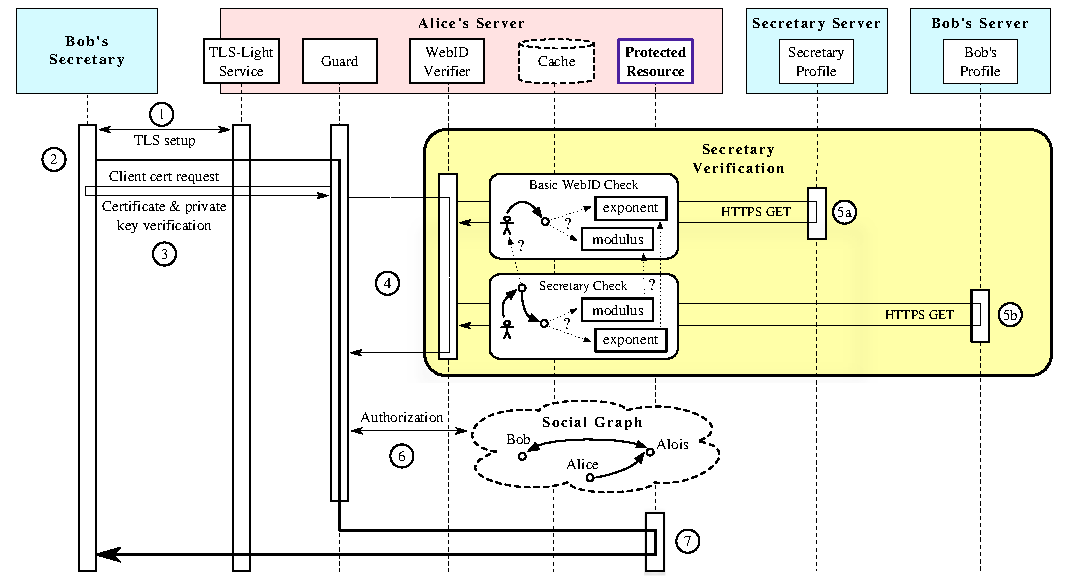
\includegraphics[width=\textwidth]{AuthSequence}
  \caption{Extended WebID authentication sequence}
  \label{fig:AuthSequence}
\end{figure*}

The following enumeration describe each authentication step in detail but concentrates on the context of access delegation:

\begin{enumerate}
    \item Bob's secretary agent opens a TLS connection with the server of the protected resource.
    \item Once TLS is set up, the HTTP request is sent to the server (e.g. a \verb!HTTP GET!) to consume or manipulate a resource.
        Here our first addition comes into play, the HTTP request header to claim an request as a secretary.
        We assume that the guard intercepts this HTTP request, and requests for a client authentication (using the TLS service)
    \item This authentication request is done using public key cryptography, sign a token with the guards private key and have the secretary send its certificate.
        This is defined in the TLS protocol which is specified in \cite{dierks-t-2012--a} and its successive RFCs.
        At the end of this step, the secretaries certificate is handled back to the guard.
    \item The guard ask the verification agent to verify the WebID is named in the certificate.

        %The WebID Certificate is then passed on to the Guard with the proviso that the WebIDs still needs to be verified.
    %The Guard then must ask the Verification Agent to verify that the WebIDs do identify the agent who knows the given public key.
    %The WebID is verified by looking up the definition of the URL at its canonical location. This can be done by dereferencing it. The Verification Agent must extract the public key and all the URI entries contained in the Subject Alternative Name extension of the WebID Certificate. A WebID Certificate may contain multiple URI entries which are considered claimed WebIDs at this point, since they have not been verified. The Verification Agent may verify as many or as few WebIDs it has time for. It may do it in parallel and asynchronously. However that is done, a claimed WebIDs can only be considered verified if the following steps have been accomplished successfully:
        %If the WebID Verifier does not have an up to date version of the WebID profile in the cache, then it must dereference the WebID using the canonical method for dereferencing a URL of that scheme. For an https://... WebID this would be done using the [HTTP-TLS] protocol.
        %The returned representation is then transformed into an RDF graph as specified in Processing the WebID Profile
        %That graph is then queried as explained in Querying the Graph. If the query succeeds, then that WebID is verified.
    %With the set of verified WebIDs the Guard can then check its access control rules using information from the web and other information available to it, to verify if the referent of the WebID is indeed allowed access to the protected resource. The exact nature of those Access Control Rules is left for another specification. Suffice it to say that it can be something as simple as a lookup in a table.
    %If access is granted, then the guard can pass on the request to the protected resource, which can then interact unimpeded with the client.
\end{enumerate}


\lstinputlisting[
    lastline=12,name=webid,style=turtle,float=htb,label=listing:webid1,
    basicstyle=\ttfamily\scriptsize,
    caption={Minimal WebID profile including a public key}
]{Listings/webid1.ttl}

\lstinputlisting[
    firstnumber=last,firstline=13,name=webid,style=turtle,float=htb,label=listing:webiddelegation,
    basicstyle=\ttfamily\scriptsize,
    caption={Access delegation by explicitly and implicitly identifying agents or application},
]{Listings/webid1.ttl}

\lstinputlisting[
    name=schema,style=turtle,float=htb,label=listing:schema,
    basicstyle=\ttfamily\scriptsize,
    caption={Schema description of the delegation property},
]{Listings/schema.ttl}



\section{Evaluation}\label{sec:eval}

\bibliographystyle{IEEEtran}
\bibliography{webid}

\end{document}
